\section{Method}
\label{Method}

\subsection{Databases}

Data for the present study originates from the “Diabetes and Lifestyle Cohort Twente” (DIALECT). DIALECT is an observational cohort study performed in the  Ziekenhuis Groep Twente (Netherlands) and is designed to investigate the effect of lifestyle and dietary habits as well as pharmacological treatment on outcomes in patients with T2D \cite{gant2017integrated}. The study included adult male and female patients with T2D (\textit{N=76}) who were monitored with a CGM system, a physical activity tracker, and kept dietary entries for up to 14 days, and only those with complete data on all three parameters for at least 5 days, along with baseline clinical patient information, were included in the analysis. Monitoring is conducted under free-living conditions at home. Blood glucose measurements every 15 minutes were recorded using the Abbott FreeStyle Libre as the CGM system, and after two weeks, the readers were returned, and the collected data were checked and uploaded. For physical activity tracking a non-invasive Fitbit wristband that measures every minute was used. During the two weeks of glucose measurements, patients were requested to maintain a food diary, which included details of the time, type, and quantity of food intake during those days.
This study was performed according to the declaration of Helsinki. Written informed consent was obtained from all patients before participation. The study has been approved by the local institutional review boards (FERB, Filed number: 22-1863) and is registered in the Netherlands Trial Register (NTR5855).

\subsection{Pre-Processing} \label{Pre-Processing}

For each patient the monitored days were divided into 24-hour periods, each of them starting at 6:00 am. This starting time is selected based on a visual inspection of the daily profiles and the average breakfast time. Daily profiles were further divided into day-time and night-time. Night-time was defined from 12:00 pm to 6:00 am to exclude the impact of the postprandial excursion after dinner and breakfast. For the feature extraction process, day-time is further divided into separate time intervals of 60 minutes from 4:00 pm until the pre-defined bedtime (12:00 pm) and an additional interval from 6:00 am to 4:00 pm. Daily profiles were excluded if multiple timestamps were missing in one of the time intervals during that 24-hour period. Further exclusion criteria are less than 50 steps completed and two or more missing timestamps for meals consumed in a single day, resulting in a total of \textit{N=713} daily profiles.

The occurrence of NH was defined when a patient spent at least a single measurement below 3.9 mmol/L (70 mg/dL), also known as level 1 hypoglycemia \cite{federation2021idf}, during night-time. The corresponding daily profiles were then labeled as nights with hypoglycemia and in all other cases as nights without hypoglycemia. 

\subsection{Feature extraction} \label{Feature extraction}
A total of 72 features were hand-crafted from CGM data, dietary entries, physical activity data, clinical patient information, and temporal-domain information. 

CGM-related features were extracted from each interval and for the full day-time. No features were included from CGM measures during night-time as the goal of this study was to predict the risk of NH in T2D patients before bedtime. First, descriptive statistics of the measured glucose concentrations were conducted for each interval and the full daytime. The assessed measures were the mean, standard deviation, minimum value, and maximum value. Further, occurrences of hyperglycemia- and hypoglycemia events over the day were extracted. Several indices of glucose variability and glycaemic control were assessed, which are commonly used in diabetology \cite{broll2021interpreting} including low- (LBGI) and high blood glucose index (HBGI), time in range, hyper- and hypoglycemia index, Glycaemic Risk Assessment Diabetes Equation (GRADE), and Glucose Management Indicator (GMI). All extracted indices have shown to be effective in predicting NH in diabetes patients \cite{sampath2016glycemic}. Further, three features were extracted based on slope coefficients from ordinary least square regressions with the purpose of gaining insights into the patterns and trends of glucose levels. Overall, this resulted in a total of 45 CGM-related features.

Next, 6 dietary features were extracted, including the sum of carbohydrate-, fat-, and calorie intake over the whole day. Past research showed that regarding food intake, the amount of carbohydrate intake has the strongest impact on the risk of NH \cite{hovorka2004nonlinear, bertachi2020prediction}. To account for the decreasing effect of carbohydrate intake on the blood glucose level a physiological model is applied. The carbohydrate onboard model (COB) \cite{hovorka2004nonlinear} was used on all meals ingested during the daytime, resulting in a single cumulative value representing the estimated remaining carbohydrates in plasma at bedtime. Last, the number of distinct meal times over the day is assessed as well as the time of the last meal before bedtime. 

Physical activity features include the total number of steps performed over the day and a feature obtained by applying the activity onboard model (AOB) \cite{oviedo2019minimizing}. This feature represents the accumulated effect of steps taken that day on the blood glucose level evaluated at bedtime. Dietary and physical activity features were defined as lifestyle features in this study and account for 8 features.

Several patient-related characteristics were extracted. These features were measurements at baseline including Hemoglobin A1c (HbA1c) values, patients' height, weight, sex, body mass index (BMI), age, and diabetes duration. Also, medical information like the type of medication (e.g. fast-acting insulin) and the doses prescribed were included as features, resulting in a total of 17 features.

Lastly, two temporal-domain features were included containing information about the day of the week and a distinction between weekends and work days. For a full description of all extracted features, see Supplementary Material \ref{tab:sup_1}.

\subsection{Feature Selection} \label{Feature Selection}
To select the most informative features for the model, a three-fold approach was employed including Mutual Information (MI) \cite{meyer2008information} criteria, Boruta feature selection \cite{kursa2010feature}, and expert knowledge.

MI is a model-independent method that captures non-linear relationships and interactions among features, thus, avoiding bias toward a particular model. MI quantifies the degree of dependence between two variables based on how much information they share, which for this study involves the comparison of their entropies. A threshold of 0.01 was applied to the MI values to identify features with meaningful associations with the target variable and avoid overfitting.

Boruta is a wrapper method incorporating an RF model. Boruta compares the importance of each feature with that of randomized shadow features to identify a relevant subset. Features with significantly higher importance based on mean decrease accuracy measure compared to their shadow features were considered relevant, while features with lower importance were considered irrelevant and removed in an iterative process. If the same variables were selected by both MI and Boruta, they were included in the final feature set as these features have been identified as important across both approaches.

The last step involved incorporating expert knowledge, where domain expertise and applicability of features in practice were considered. Furthermore, this step allowed for the inclusion of variables that may have demonstrated exceptional performance within one of the methods (MI or Boruta), but may not have met the threshold or importance criteria of the other method. 

By integrating these three steps, the feature selection process aimed to capture the most informative features for the predictive modeling task in a robust and unbiased manner, while also considering expert knowledge for interpretability and clinical relevance. 

This process is applied to the full data condition and also to the Lifestyle condition. For the full data condition, a feature space of 41 variables was selected and for the Lifestyle condition, 18 features were selected. The most important features based on the Boruta approach for each data condition are presented in Figure \ref{fig:features}.

\begin{figure}[tb]
\centering
\caption{Feature Importance values of 10 most important features for two conditions.}
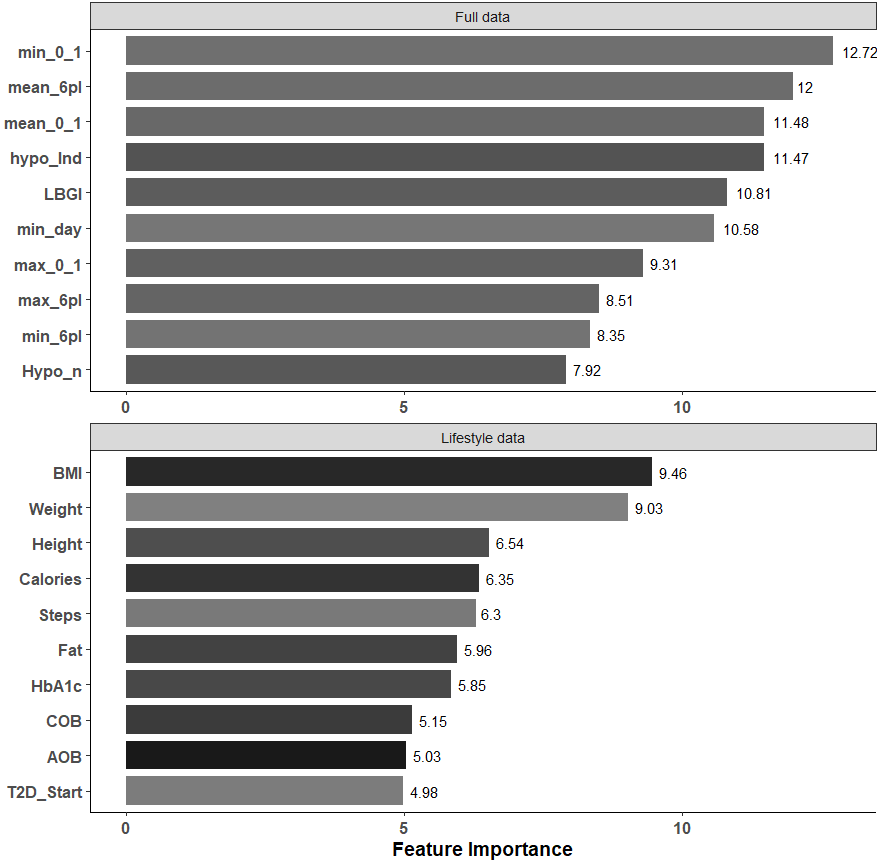
\includegraphics[width=0.5\textwidth]{Figures/Feature_Imp_rs.png}
  \parbox{0.45\textwidth}{\small{\textit{Note:} Abbreviations are explained in Supplementary Material \ref{tab:sup_1}. Feature Importance values are based on the mean decrease accuracy measure based on Boruta feature selection .}}
\label{fig:features}
\end{figure} 

\subsection{Machine Learning Algorithm Selection}  \label{Machine Learning Algorithm Selection}

To determine the best-performing model for the specific data characteristics, multiple ML algorithms were applied, including Random Forest (RF), Support Vector Machines (SVM), eXtreme Gradient Boosting (XGB), and Lasso logistic regression (Lasso). These algorithms were selected as they have been successfully used in previous studies for hypoglycemia prediction \cite{zhang2023data}.

RF is known for its ability to handle overfitting and has been used in multiple studies predicting hypoglycemia \cite{kodama2021ability,athey2019generalized}. SVMs are effective in high-dimensional datasets, can model nonlinear relationships between variables, and handle imbalanced data \cite{smola2004tutorial}. XGB is particularly successful in handling imbalanced data \cite{mujahid2021machine} and Lasso is useful for high-dimensional data as it performs another feature selection by shrinking the coefficients of less important features to zero \cite{kodama2021ability}.

The classifiers selected for this study were chosen for their ability to be integrated into decision support systems. All chosen ML algorithms have been shown to be accurate, transparent, interpretable, and computationally efficient, which makes them well-suited for practical applications \cite{mujahid2021machine, kodama2021ability}.

\subsection{Model Building Process} \label{Model Building Process}

\subsubsection{Model building preparation} \label{Feature category}
Class imbalance is a prevalent issue in the prediction of NH \cite{guemes2019predicting,parcerisas2022machine}, as observed in this study where only a small fraction of the recorded nights exhibited hypoglycemic events, leading to a bias towards the majority class. To address this issue, Up-sampling, Synthetic Minority Over-sampling Technique (SMOTE) \cite{chawla2002smote}, and cost-sensitive learning using threshold moving \cite{ling2008cost} were employed. Up-sampling involves replicating the minority class to balance the number of cases in each class. SMOTE generates synthetic samples of the minority class by interpolating between the minority class cases and their nearest neighbors, which has a lower risk of overfitting compared to Up-sampling. Both resampling strategies were employed on the training set only, as the test set should reflect the real-world distribution of the classes.

Cost-sensitive learning is applied to handle the varying costs of misclassification errors using threshold moving. The optimal threshold is chosen to be the point closest to the top-left part of the Receiver Operating Characteristic (ROC) curve with the highest sensitivity (SENS) or specificity (SPEC).
Within the threshold moving process, this study employed an increased weight to false negatives (FN), which refer to falsely classifying a night with hypoglycemia as a night without, compared to false positives (FP), which refer to falsely classifying a night without hypoglycemia as a night with. This weight was set to be twice the relative cost for an FN compared to an FP, which is in line with common clinical practice \cite{ling2008cost} as the cost of FN may lead to more consequences than the cost of FP.

Additionally, features are scaled to have a mean of zero and unit variance.

\subsubsection{Data split \& Cross-validation} \label{Data split}
The data was split into 25\% for testing and 75\% for training. To optimize the models' performance, 10-fold cross-validation was performed for the training set. This process was repeated for three folds of training data with different divisions of training and test data to overcome bias due to the small sample size. Mean and standard deviations (SD) over the three folds for the evaluation metrics were reported. Each ML algorithm was trained separately with different hyperparameter tuning strategies. Grid search with default values from the \texttt{caret} package \cite{kuhn2020package} for each ML classifier was used as a baseline, followed by a random search to broaden the search space of the hyperparameters. Additionally, a customized grid search was applied based on the best results of the first two searches and recommendations of search spaces from Probst et al.\cite{probst2019tunability}. Both SMOTE and Up-sampling techniques were applied during the cross-validation procedure to reduce bias in the sampling process. 

All tuning processes were applied to the original dataset, as well as to the up-sampled and SMOTE-generated datasets. The entire process, including data splitting, resampling, and model training, was repeated for both data conditions (Full data condition \& Lifestyle condition).

\subsection{Evaluating Model Performance} \label{Evaluating the Performance}
To evaluate the performance of the ML algorithms, widely-accepted evaluation metrics were used, such as SENS, SPEC, and AUC. 
    
\begin{center}
\begin{minipage}{0.25\textwidth}
\centering
\begin{equation}
\text{SENS} = \frac{\text{TP}}{\text{TP} + \text{FN}},
\label{eq:sens}
\end{equation}
\end{minipage}
\begin{minipage}{0.25\textwidth}
\centering
\begin{equation}
\text{SPEC} = \frac{\text{TN}}{\text{TN} + \text{FP}}.
\label{eq:spec}
\end{equation}
\end{minipage}
\end{center}

As shown in equation (\ref{eq:sens}), true positive (TP) represents that nights with hypoglycemia were correctly identified as hypoglycemic, and FN represents that nights with hypoglycemia were incorrectly identified as non-hypoglycemic. Therefore, SENS measures the proportion of positives (NH) that are correctly classified. In equation (\ref{eq:spec}), true negative (TN) represents that nights without hypoglycemia were correctly identified as non-hypoglycemic, and FP indicates that nights without hypoglycemia were incorrectly identified as hypoglycemic. Hence, SPEC shows the proportion of negatives (no NH) that are correctly identified.

Additionally, the AUC measures the ability of classifiers to distinguish between positive and negative cases across all possible classification thresholds. AUC is particularly useful when dealing with class imbalance as it is not affected by the threshold used to make predictions. Therefore, also not being affected by the applied cost-sensitive learning approach as it is independent of the threshold selection.

\subsection{Software} \label{Software}
Analyses and pre-processing are performed using \texttt{R version 4.2} \cite{team2020rstudio}. Model training and feature selection are conducted with the \texttt{caret} package. Class imbalance is handled with the \texttt{DMwR} package. Packages used for ML algorithms are \texttt{ranger} for RF, \texttt{kernlab} for SVM, \texttt{xgboost} for XGB, and \texttt{glmnet} for Lasso.